\documentclass[a4paper]{article}

\usepackage[english]{babel}
\usepackage[utf8]{inputenc}
\usepackage{amsmath}
\usepackage{graphicx}
\usepackage{listings}
\usepackage[colorinlistoftodos]{todonotes}

\lstset{
	language=python
}

\title{Assitive Device for Hand Amputees: \\ Dumper Robot}

\author{CS321: Project Report - Part II \\ Group 19}

\date{\today}

\begin{document}
\maketitle

\section{Introduction}
\label{sec:introduction}

The \textbf{Assitive Device for Hand Amputees} system has been created with the motive of enabling people with both arms amputated interact with the physical and the digital world in a convenient manner. To this end, we have different modes present that allow the user to work with a computer's keyboard and mouse pointer, and the physical world. In particular, the physical mode allows the person to control a dumper robot through hand gestures alone. This document is a detailed discussion of the design, construction, operation and flaws of the dumper robot. It is lucid enough to serve a user manual and technical enough to serve as a technical manual for troubleshooting, while also describing the processes we used for achieving the final product.

\section{Design And Construction}

This section describes some of the design philosophy of the bot, as well the choice of materials and alternates that can be used to create the chassis. Fig. \ref{fig:bot_design} shows the design (bottom view) that was finally adopted, and the different components that were used.

\begin{figure}
\label{fig:bot_design}
\centering
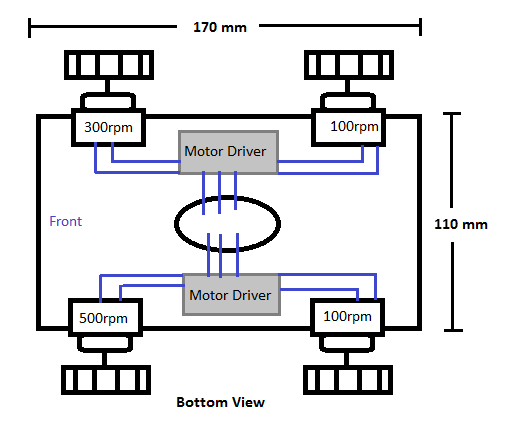
\includegraphics[width=0.75\textwidth]{bot_bottom.png}
\caption{Bottom View of Dumper Robot}
\end{figure}

\subsection{Design}

\begin{description}

\item[Chassis] The dumper robot has been designed be capable of transporting moderately heavy loads (in the order of 5-8 kilograms, such as a stack of books, or a laptop with all its accessories) and yet be light enough to be transported manually if required. With this in mind, the different options available to us for creating the base plank of the chassis were \textit{plywood, sheet metal, acrylic sheet} and \textit{balsa wood}. The plywood that was available was around 10mm thick, and hence too heavy to be used. On the other hand, acrylic sheets would have served well in the weight department, but are generally brittle and capable of splintering when subject to heavy loads or on collision with other objects. Hence, sheet metal and balsa wood were the plausible options. We chose to go with \textbf{balsa} as we also wanted to drill a hole in the base plank so that we could cleanly pass wires between the two sides.

\item[Drive Wheels] We had to decide between constructing either a 2-wheeled bot with a castor wheel for balance, or a 4-wheeled bot. While a 2-wheeled bot is easier to maneuver, construct and operate, it might not fare well over different kinds of terrains (such as a slippery floor, a tiled floor, etc). Also, the load that can be transported is also lesser (for the same kind of motors and the same bot construction). On the other hand, the 4-wheeled design would excel in both different terrains as well as load-bearing capacity, but would be bulkier, would require more effort for construction and might not be as maneuverable. We decided to go with the \textbf{4-wheeled design} in an attempt to increase the carrying capacity of the bot.

\item[Loading Area] The possible designs we considered with respect to the loading area were: a 2-level bot, with the breadboard, Arduino and drivers on the first level and the second level used for putting weights; a single-level bot but with a slightly raised `stage' for placing loads; and a single-level bot with all the weights placed adjacent to the breadboard/Arduino. The last approach did not offer much room for loads, the second option also would result in a very cluttered stage area (which would make debugging and maintenance difficult). Also, the bot might be subjected to jerks when starting or braking (due to difference in weight distribution) in the second approach. Hence, we choose the first approach as it provided sufficient space for placing loads even though it increased the weight of the bot itself.

\item[Processing and Communication] Communication with the user's device was achieved through the use of \textbf{wireless communication} via the XBee Module. An \textbf{Arduino Uno} has been used for processing, primarily due to its small size and its availability. More powerful processors such as Raspberry-Pi or Intel Galileo have been avoided, as they would have been overkill for this project. The processing at the bot's end is minimal, and hence can be accomplished through use of the 16MHz Uno. Other than wireless, we also tried using I2C communication and serial communication between the Uno and the user's Arduino Mega.

\item[Power] Naturally, the dumper bot had to be mobile and maneuverable, and hence we decided to use a portable power supply that was capable of powering the Arudino, the motor drivers and the wireless modules as well. In this case, we used a \textbf{12V Lithium-Polymer battery} with a rating of 2200mAh. 

\item[Control Strategy] Most of the control strategy is explained in Part I of this documentation. We reiterate once more that the strategy has been chosen to minimize user discomfort, and provide large tolerances to error. For example, we've chosen to support only a 90$\deg$ turn to the left or right, to improve error tolerance.

\end{description}

\subsection{Materials Used}

The components used to make up the dumper robot are as follows:

\begin{itemize}
\item{Motor Drivers:} We used 2 motor driver chips manufactured by Nex Robotics, which had the L293D driver IC mounted on a board and integrated with a heat sink. Each IC is capable of powering 2 motors at a time through a 12V source, and is signalled by the Uno (using a 0-5V digital logic). The drivers were mounted on the underside of the base plank.

\item{Motors:} Due to insufficient availability, we used 4 DC motors of varying speeds. The back wheels are powered by 2 100rpm DC motors, while the front left wheel is powered by a 500rpm DC motor and the front right wheel is powered by a 300rpm DC motor.

\begin{figure}
\centering
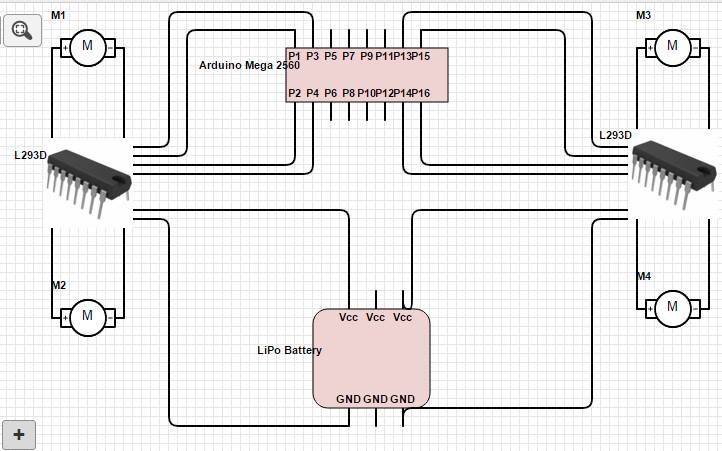
\includegraphics[width=0.75\textwidth]{electric_schema.jpg}
\caption{Motor Driver Connections}
\end{figure}

\item{Arduino Uno:} A 16MHz Arduino Uno with 14 digital I/O pins, one serial port, one I2C interface and an operating voltage of 5V was used for processing. It was mounted on the topside of the base plank.

\item{XBee Wirelee Module:} A 2.4GHz XBee module using 802.15.4 stack (the basis for Zigbee), a 3.3V operating voltage and a serial command set was used for establishing wireless communication. An XBee-Arduino shield was used for interfacing the XBee with the Arduino. Note that the shield has an operating range of 300 feet.

\item{Battery:} A 12V LiPo battery pack with a power rating of 2200mAh was used for powering the Arduino and the motor drivers.

\item{Wheels:} Four plastic, rubber-tired wheels with a diameter of 4cm are mounted on the motor shafts and are attached using screws.

\item{Chassis:} The chassis was constructed out of a 170mmx110mm plank of balsa wood, with an elliptical hole in the middle to allow the passage of wires. The secondary level was constructed out of a cardboard enclosure.

\item{Miscellaneous:} Numerous wires, jumpers, L-joints and a breadboard were used.
\end{itemize}

\subsection{Construction}

Construction of the bot was done in a bottom-up manner. We first made the chassis out of balsa wood having a dimension of 170mm by 110mm. We used a chisel to carve out an elliptical hole with the axes being roughly 30mm by 7mm. Next, we mounted the wheels onto the motor shafts, and used L-joints to affix the motors to the base plank. Next, we used double-sided tape to fix both the motor drivers to the underside of the base plank, and made the appropriate connections between the motor wires and the drivers (this involved soldering some of the wires as well). 

All motor related wires were taped to the underside to ensure clean construction and easy debugging. The remaining control wires were passed through the elliptical hole to the topside of the plank, where they were interfaced with the Arduino. The Arduino itself was affixed (using double-sided tape) to the front topside half of the plank, and the breadboard to the rear topside half of the plank. The XBee module was interfaced with the Arduino via a shield. Finally, all wires were taped down to avoid loose ends.

During the construction, we tried to be as clean and efficient as possible. This included using wires of exactly the required length, using color-coding to distinguish between wires, wiring together relevant groups of wires to create a bus and choosing the positions of the different components carefully. This helped as tremendously in the later stages, during debugging and maintenance of the bot.

\section{Control and Operation}

This section describes the control and operation aspects of the bot. We cover the techniques used for making the bot operational, any drawbacks that may be present and ways in which they can be resolved. Programming of the bot was done through the Arduino IDE in the C programming language.

\subsection{Control}

\begin{description}
\item[Skid Steering] Skid steering is a driving mechanism implemented on vehicles with either tracks or wheels which uses differential drive concept. Similar to differential drive, this method engages one side of the wheels and turning is done by generating differential velocity at opposite side of a vehicle, as the wheels in the vehicle are non-steerable. In fact, the only difference between the two methods is that in Skid Steer drive, the balancing castor of a bot is replaced with two driving wheels. This method is particularly useful as it provides greater traction and is especially good for rough terrain. However, driving in a straight path is a hard to achieve task as both the motors are expected to drive at exactly the same speed. This can still be taken care by other sensing devices, but adds cost and control mechanisms.

\item[I2C and Serial Communication] The bot is capable of using either I2C or serial communication if wired communication is necessary. I2C communication is established by using the A4/A5 pins of the Arduino Uno as the SDA/SCL ports, and by using the Wire library (standard part of Arduino API). However, it must be noted that the I2C standard stipulates that the master bus be used by exactly one device at a time, in order to prevent distortion of the transmitted signal. Similarly, the RX/TX ports of the Uno were used to achieve serial communication, and the Serial library (again, a part of the standard Arduino API) has been used.

\item[Wireless Communication] Wireless communication uses the XBee module. In our case, we used an XBee-Arduino shield to make interfacing convenient. The Xbee was powered by the 3.3V pin of the Arduino, and the D0 channel of DIN/DOUT pins (data in/data out) were used for communication. The other end of the channel was connected to the RX/TX ports of the Uno, and the Serial library was used. It is possible to work without using the default hardware serial ports, through usage of the SoftwareSerial library (which converts a GPIO pin to a serial pin).

\item[User Interaction and Control] The Arduino was programmed to respond to user interaction and carry out the assigned tasks. Specifically, after sending an initialize signal, the user's device transmits motion instructions to the bot through pre-defined codes. As explained in Section 2, we have chosen to implement front, reverse, left and right as the only valid motion commands. This ensures a large error margin, and hence allows greater range of movement to the user.
\end{description}

\subsection{Operation}

The dumper bot is manual, in the sense that the by itself, the bot will not undertake any actions. Rather, it will wait for user stimulus to dictate its actions. Hence, most of the operation procedures and the design philosophy behind them are covered in Part I of the documentation, which describes the user's end of the system. 

\section{Drawbacks and Improvements}

\begin{description}
\item[Chassis Integrity] By itself, the bot weighs around 1-1.5 kilograms. While the chassis is sturdy enough to handle weights of the order of 5-8 kilograms. This might be an issue in case of heavier loads and might reduce the utility of the bot. In this regard, a sheet metal chassis might hold up better to loads.

\item[Mobile Power Supply] While we have used a 12V Li-Po battery for demonstration purposes, any practical usage of the bot will warrant a stable and rechargable power supply. Wall-socket rechargable batteries, lead-acid batteries and solar panels may all be viable alternatives.

\item[Drift Control] Currently, the bot has a tendency to drift off-course by a few centimeters every meter, when operated in forward mode. This is a by-product of using the skid steering technique (as mentioned in Section 3) and of having motors with different speeds. This can be rectified by the use of an error correction technique, such as Proportional-Integral-Derivative(PID) or a Kalman filter.

\item[Wireless Communication Range] With a range of around 300 feet, the XBee module is sufficient for indoor environments (such as small houses, classrooms, etc.) but might not be very effective for larger distances. Usage of long-range communication devices might help in this regard.
\end{description}

\section{Conclusion}

The dumper robot constructed as part of the Assitive Device for Hand Amputees System is useful tool for transportation of moderately heavy loads, such as those encountered in everyday life (books, groceries, laptop, bag). As such, it can prove to be an immensely helpful tool for hand amputees. A stable, rechargable power source and greater wireless range would further increase its utility.

\section{Acknowledgements}

We would like to thank Prof. S. B. Nair for giving us the opportunity to work on this exciting project. It has helped us learn more about the control-based applications of computer systems, and the sense of satisfaction we feel on having developed such a system is immeasurable. We would also like to thank Mr. Tushar Semwal for his tireless help and guidance, and Mr. Hemanta Nair for providing us with some of the equipment necessary for the completion of this project. Finally, we would like to thank the Manas and Barak Hostels' Technical Secretaries for providing much of the equipment used in construction of the dumper robot.

\end{document}